\subsection{Conditioned-Target Object Detector}
\label{sec:cond_target_obj_detector}
In this section, we will introduce the architectural design dedicated to the \textit{command analysis task}. We explicitly aim to identify the target object position in the image space by predicting its bounding-box $bb_{t}^{target}$. This prediction is made through a parametrized function denoted as $\mathcal{F}_{\psi}$ that takes in input the current agent observation $s_{t}$ and the command representation $c_{m_{i}}$, i.e., $bb_{t}^{target} = \mathcal{F}_{\psi}(s_{t}, c_{m_{i}})$. In the realm of Computer Vision, Object Detection is a well-established and extensively researched problem, with modern methods achieving high levels of performance in detection and classification tasks. However, we cannot directly apply the methods employed in previous work \cite{jiang2023vima, zhu2023viola}. This is because our objective is not to detect all objects in the scene, but our focus is on identifying the ``target object", which can vary depending on the specific task variation at hand. Furthermore, we aim to design a method that is agnostic to object categories, meaning it doesn't need to answer the question, ``What category does the object belong to?" Instead, its primary goal is to answer, ``Where is the target object located?" This approach enables the method to be easily adapted to scenarios where multiple object categories are present.
\newline To address this task, we drew inspiration from the ``Visual Question and Answering" problem \ref{sec:research_activity}. Our approach is rooted in the concept that, much like the architecture presented in \cite{perez2018film} can direct attention to specific regions of an image in response to input queries, we aim for our model to exhibit a similar ability. Specifically, we want the model to focus on a particular portion of the image based on the task command $c_{m_{i}}$.
The proposed architecture is reported in Figure \ref{fig:ctod}
\begin{figure}[htb]
    \centering
    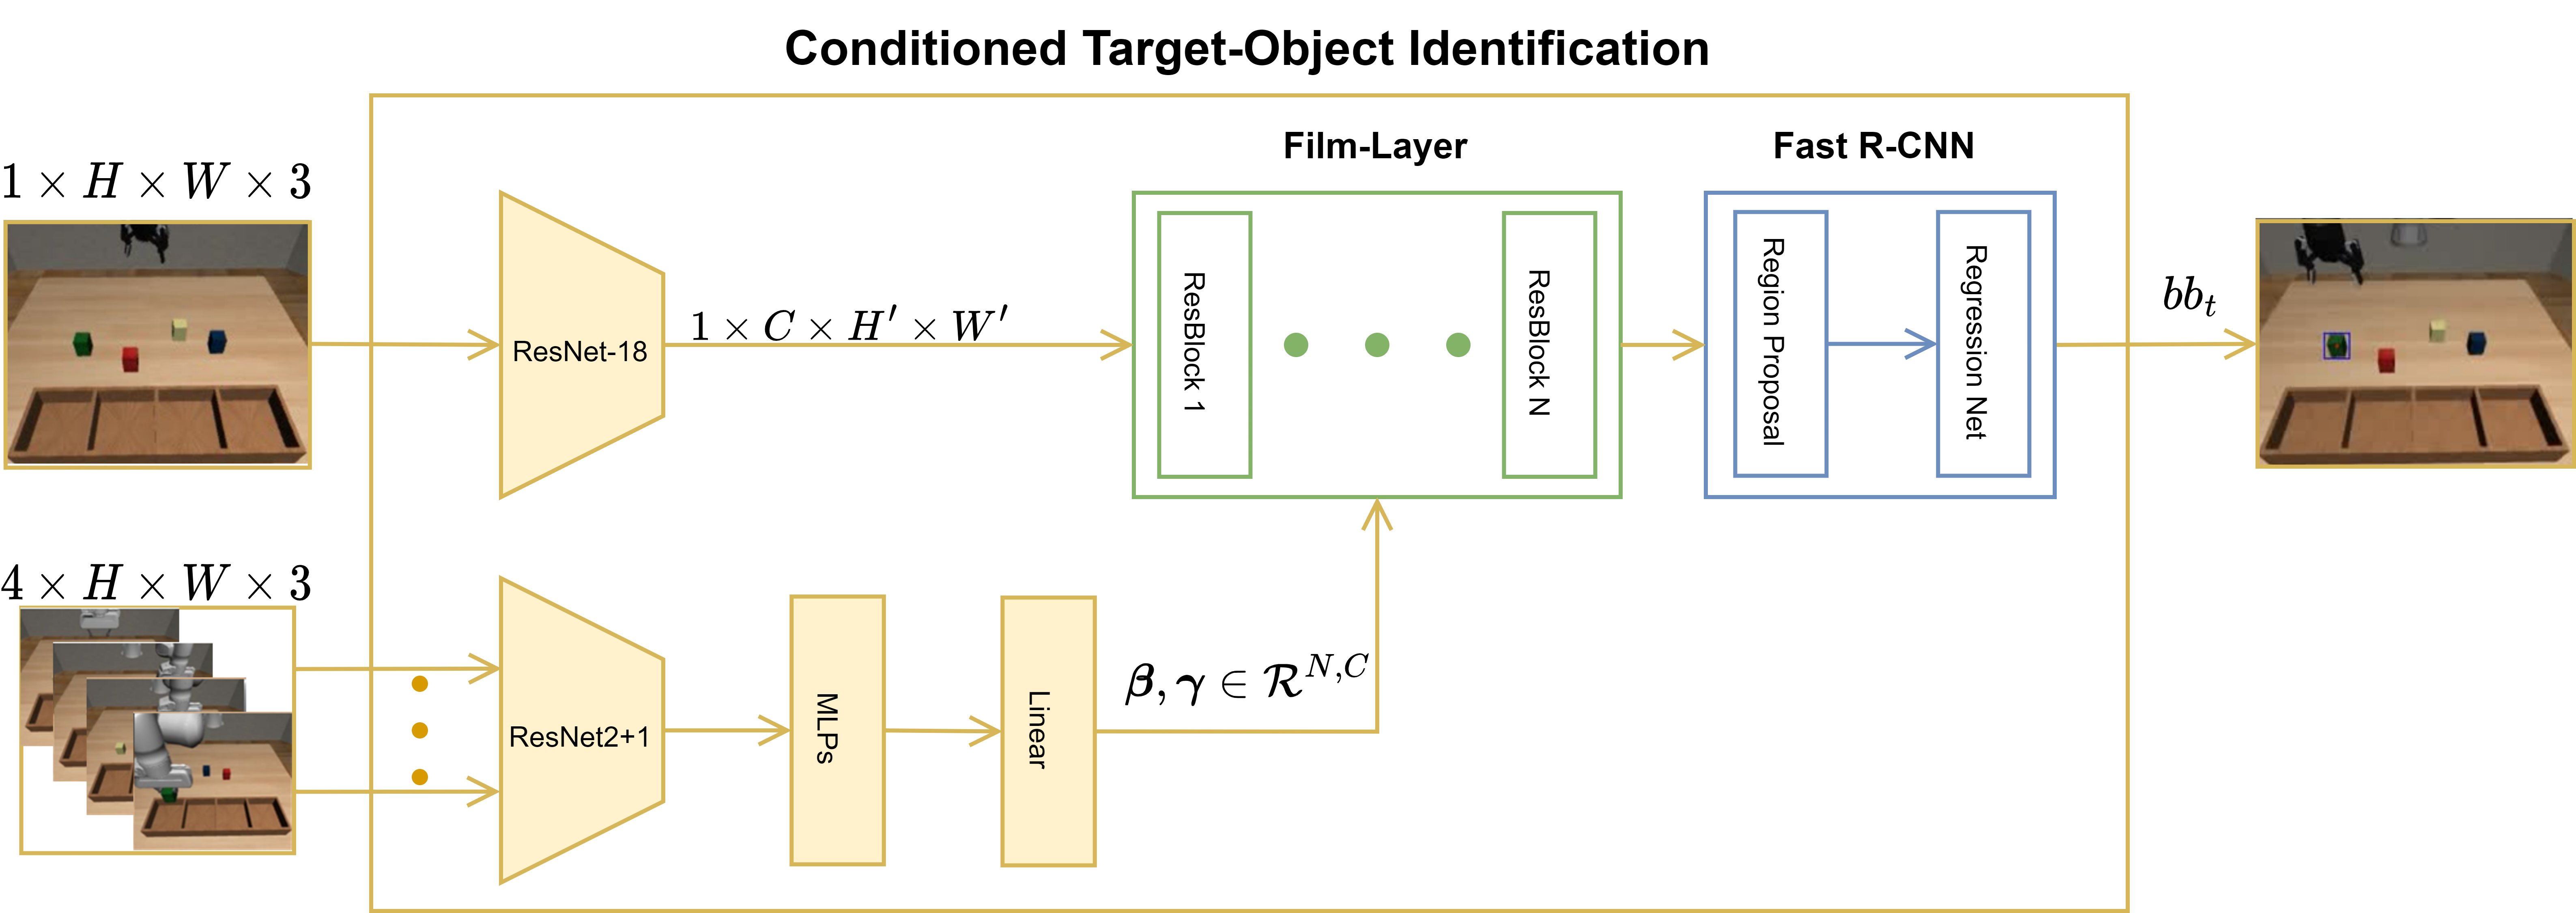
\includegraphics[width=0.8\textwidth]{Figures/images/ctod/ctod.png}
    \caption{Proposed architecture for solving the Conditioned-Target Object Detector}
    \label{fig:ctod}
\end{figure}

It is composed by the following modules:
\begin{itemize*}[label=$(\bullet)$]
    \item \textit{ResNet-18} \cite{resnet}, as feature-extractor for the agent observazione $s_{t} \in \mathbb{R}^{H \times W \times 3}$, rapresented as an RGB image;
    \item \textit{ResNet2+1} \cite{resnet21},  as a feature extractor for the command description $c_{m_{i}} \in \mathbb{R}^{4 \times H \times W \times 3}$. This description is represented by a set of 4 frames sampled from the demonstrator's execution video. The chosen architecture facilitates the extraction of both spatial and temporal features. Subsequently, the generated features are flattened and processed through a Multilayer Perceptron (MLP) network;
    \item The FiLM-Layer, as introduced in \cite{perez2018film}, serves as the module responsible for integrating the features derived from both the agent and command processing stages. In detail, this layer carries out a modulation of the $c^{th}$ activation through a feature-wise affine transformation, expressed as $FiLM(\textbf{F}_{c}|\gamma{c}, \beta_{c}) = \gamma_{c} \textbf{F}_{c} + \beta_{c}$. Here, $\gamma$ and $\beta$ represent parameters generated by the linear module, based on the desired input;
    \item \textit{Fast R-CNN} \cite{fastrcnn}, is the dual-stage anchor-based object-detector, that has to infer the bounding box position based on the features maps generated by the previous module.
\end{itemize*}
The whole architecture has been trained according to the classic object-detector loss-function $\mathcal{L} = w_{1}\mathcal{L}_{reg} + w_{2}\mathcal{L}_{cls} + w_{3}\mathcal{L}_{class}$, where: \begin{itemize*}[label=$(\bullet)$]
    \item $\mathcal{L}_{reg}$ is the \textit{L1-loss} function that compares the predicted bounding-box offset and the ground truth offset;
    \item $\mathcal{L}_{cls}$ is a \textit{binary-cross entropy loss} that allows the model to learn the difference between foreground and background bounding-box;
    \item $\mathcal{L}_{class}$ is a cross-entropy loss designed to accommodate object classification. In our scenario, owing to the class-agnostic nature of our model, we trained it to distinguish between two object classes: \textit{target} and \textit{no-target}.
\end{itemize*}
\begin{table}[htb]
    \centering
    \fontsize{11pt}{11pt}
    \selectfont
    \caption{Conditioned-Target Object Detector performance}
    \label{table:ctod_performance}
    \resizebox{\linewidth}{!}{%
        \begin{tabular}{>{\centering\hspace{0pt}}m{0.304\linewidth}>{\centering\hspace{0pt}}m{0.335\linewidth}>{\centering\arraybackslash\hspace{0pt}}m{0.263\linewidth}}
            \hline
            \textbf{Task} & \textbf{Precision@0.5} & \textbf{Recall@0.5} \\
            \hline
            Pick-Place    & 0.87                   & 0.99                \\
            \hline
            Nut-Assembly  & 0.96                   & 0.99                \\
            \hline
        \end{tabular}
    }
\end{table}

The model's performance is documented in Table \ref{table:ctod_performance}. To validate the module we follow the test procedure explained in Section \ref{sec:baseline_definition} but moving the robot with the manually defined control rules used to collect the simulated dataset. It is evident that we have achieved a highly stable detector in terms of both precision and recall. This stability is maintained throughout various phases, encompassing the initial frames when the robot approaches the target object and during the manipulation itself. For a quantitative analysis of prediction distribution in both pick-place and nut-assembly scenarios refer to Table \ref{table:ctdo_prediction_distribution}. It's worth noting the remarkably low number of false-negative predictions, that indicate frames for which the model does not predict any bounding-box for the target object. About the false positive cases, for the pick-and-place task, the system predicts a bounding box for the target object that is completely non-overlapping with the ground truth only 192 times out of 625, and 52 times out of 186 for the nut-assembly task. In all other cases, we have an Intersection Over Union (IoU) less than 0.5, but it still indicates that the system can identify the region of the image where the target object is located, as in the second frame of Figure \ref{fig:ctdo_trajectory_execution}. These results emphasize the effectiveness of the proposed system in efficiently handling the command analysis task, which involves precise and consistent localization of the target object. Notably, even when the demonstrator and agent scenarios exhibit variations in object configuration, our system consistently demonstrates the ability to accurately detect the target object. \hl{This achievement is made possible by the establishment of a meaningfull correlation between the current agent's observations and the command, which has been a central focal point in the proposed architecture, achieved through the usage of the FiLM conditioning layer.}\change{Possibile spiegazione dei risultati ottenuti}
\begin{table}[bth!]
    \centering
    \caption{Conditioned Target Object Detector prediction distribution}
    \fontsize{10pt}{10pt}
    \selectfont
    \label{table:ctdo_prediction_distribution}
    \begin{tblr}{
        width = \linewidth,
        colspec = {Q[185]Q[73]Q[162]Q[177]Q[162]Q[177]},
        cells = {c},
        hlines,
        hline{1,4} = {-}{0.08em},
            }
        {\textbf{Task } \\\textbf{(\#Frames)}} & \textbf{TP} & {\textbf{FP }\\\textbf{pre-picking}} & {\textbf{FP }\\\textbf{post-picking}} & {\textbf{FN }\\\textbf{pre-picking}} & {\textbf{FN }\\\textbf{post-picking}} \\
        {Pick-Place     \\(11229)}                & 9718        & 625                                  & 812                                   & 74                                   & 0                                     \\
        {Nut-Assembly   \\(5643)}                & 5187        & 186                                  & 80                                    & 10                                   & 0
    \end{tblr}
\end{table}
\begin{figure}[bth!]
    \centering
    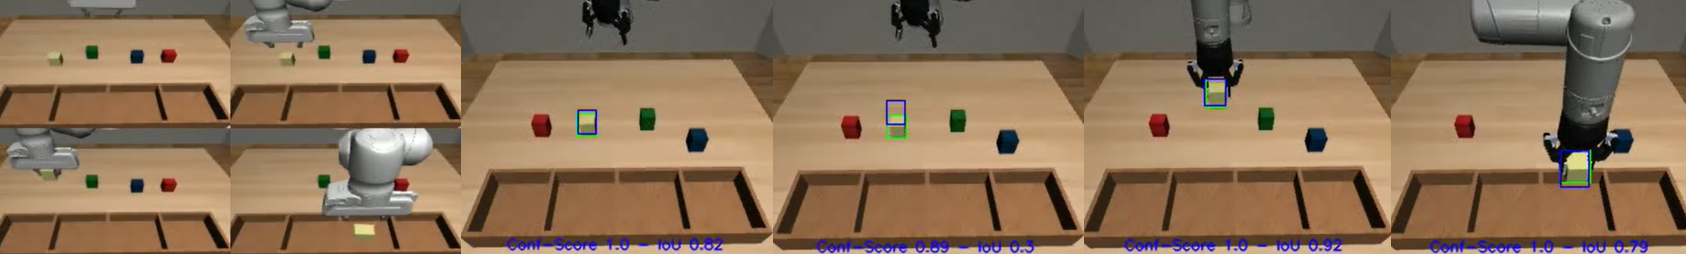
\includegraphics[width=0.9\textwidth]{Figures/images/object_detector/example_prediction.png}
    \caption{Example of predictions during trajectory execution}
    \label{fig:ctdo_trajectory_execution}
\end{figure}

